\section{為什麼無綫電視會被稱為 CCTVB?}

因為無綫電視近年的節目(特別是新聞時段)的編採方針脫離了不少人對傳媒監察權力的期望,甚至被認為變成了政府的喉舌,和中國大陸的中央電視台(CCTV)無異,所以被謔稱為CCTVB。無綫電視的問題並非獨有案例,香港傳媒的轉變和社會政治經濟結構的關係,以及對言論和新聞自由的影響,是香港近年來其中一個最重要的問題。

傳媒本身值得關注,是因為它可以影響社會輿論。它們的影響體現在四方面:首先,它們可設定議題和討論框架,帶領公眾的注意力。例如二零零六年反對清拆天星碼頭的抗議活動,示威者主張民主規劃,但傳媒關心的卻是示威者都十分年輕,而且勇於以直接行動阻擋清拆,於是社會輿論很快便被引導向「為何這一代的年輕人會以激烈手段抗爭」之上,沒有注意到他們的真正訴求。第二,它有廣泛傳播的功能,例如無綫電視的收視再差也會同一時間有數以十萬計的觀眾看到,相對來說社交網絡的帖子能有數十萬的收視已算極為成功。小眾偶像要變成全港話題,很大程度要靠傳媒的曝光機會。如是者,傳媒還有第三和第四個功能:合理化和忽視。一些本來被視為是社會禁忌的行為(視乎不同社會,可以是支持同性戀也可以是歧視少數族裔)經主流傳媒曝光後,會讓其他人覺得這些禁忌原來可以被打破,然後有樣學樣;反過來,如果傳媒刻意不提及某些觀點,認同這些觀點的人可能會以為自己只是社會中的少數,就未必願意公開承認支持這些觀點了。

正因為傳媒對社會輿論影響力大,它們特別是在政治壓力面前能否做到公平公正就十分重要。回看香港歷史,傳媒和政治的關係經歷了很多個不同階段。回到六十年代或以前,香港的中文報章受意識形態主導,成為國共對抗的虛擬戰場。政府對此並不反感,因為當輿論忙於互相攻擊就少了時間監督政府。事實上當時的香港仍處於難民社會時期,政府管治強勢而民間參與的機會十分有限,傳媒監督的空間也不多。到了七、八十年代,隨著社會變得小康,本土社會訴求和社會運動也日益增加,而政府面對中英談判也開始開放管治,傳媒的監察角色變得重要。到了八九民運和及後在香港引發的民主浪潮,香港的新聞從業員不單止成為歷史的見證者,甚至有時變成歷史的參與者,也就觸動了一整代的傳媒人決志以社會關懷為己任。

不過,當外在的政治環境在特區成立後逐漸轉變,傳媒生態和傳媒人的工作環境也變得很不一樣。學者陳韜文以「代母民主」(Surrogate Democracy)的概念來解釋特區下的傳媒角式:政治制度本身的缺陷使得正規政治(無論是政府或議會)未能代表民意,所以傳媒在香港「為民發聲」的角色就顯得十分重要,甚至比一個正常的民主社會更為重要,輿論對新聞和言論自由也更為敏感。實際上,當議會未能對政府構成實際制衡,傳媒意見領袖的批判有時會顯得更直接和有力。

特區成立早期的「峰煙節目」是本地學者的一個重要的傳媒研究案例。「峰煙」本來是英文 “Phone-in” 的音譯,即是容許聽眾打電話到直播節目中和主持人甚至是被訪者直接對話。其中最有名的要數商業電台節目《風波裡的茶杯》。由於節目能迎合市民對政府高官的不滿,加上主持人鄭經翰辛辣敢言的作風,收聽率長期高企。該節目於早上播出,而在節目中被攻擊的對象往往會成為當日新聞輿論的焦點,使得政府內部也要規定凡有任何社會熱點,官員必須於早上十時即該節目完結前發表公開回應。因此,鄭經翰獲得「十點前特首」的稱號,即節目期間他才是眾高官的真正問責者。

不過要當鄭經翰的位置並不容易。首先是他在一九九八年於往電台上班途中被襲,身中八刀,手筋被砍斷,一度垂危而要在醫院休養兩個月,輿論懷疑和他在節目中攻擊既得利益有關。到了二零零三和二零零四年期間,商台正與政府商台協商續牌,鄭經翰在休假後被突然解僱。數年後他創立了香港數碼廣播公司,可以重新主持節目,但其後又因股東爭拗而再度停播。

鄭經翰的案例經常被用作探討傳媒從業員與管理層及持有人之間的關係,如何影響傳媒發聲的空間。前中大新聞與傳播學院院長馮應謙曾詳細分析自特區成立以來香港各傳媒機構擁有權的轉變,認為親建制陣營的商人透過收購傳媒來得到好處。他們不在乎能否在這些傳媒機構賺錢,更重要的是他們可利用香港傳媒持有人的身分為在中國大陸的投資尋求保障。例如他們可以在特區政府有需要的時候,通過收緊轄下傳媒的言論尺度,甚至以連續多日頭版攻擊非建制陣營,來向中國政府表達效忠,而中國政府則在其他利益範疇予以回報。近年來傳媒易手和被質疑自我審查的案例,有《明報》、《南華早報》、《成報》和亞洲電視等。

回到無綫電視的例子,雖然香港法例規定免費電視的持牌人必須是香港永久性居民,但有分析指現時無綫電視的真正掌權者為中國大陸的國家資本。無綫電視的大股東財團,後面包括由國家開發銀行、招商局,和上海國資委持有的公司出資成立的基金。而證券及期貨事務監察委員會(證監會)的文件揭露,該基金會的董事長對財團的董事任免上絕對權力。因此,有評論認為無綫電視其實已經「染紅」,成為國家資本的一部分。

在實際操作上,無綫電視的新聞節目近年經常被評為刻意為政權粉飾太平,例如即使有大規模的遊行集會也不會放在新聞頭條或不作報道。於佔領運動期間發生的「七警案」(見問題三十)雖然是由無綫新聞揭發,但在首次播出後便被管理層要求刪減報道內容。播出當日下午,二十八名無綫電視的新聞工作者發表公開信,表明不同意管理層處理手法。及後負責第一個版本稿件的當席採訪主任被調職,而當日發出公開信的新聞工作者有一半於半年內因不同理由辭職。「七警案」只是近年來無綫電視眾多被質疑未能做到公平公正的案例之一,CCTVB的謔稱也是由此而起。

新聞審查不一定要以管理層直接指令的這種粗暴的方法發生。學者區家麟指出,很多時候一些間接的新聞審查可以更為有力,也更難被察覺和引起反感。例如管理層可利用「平衡報道」報道的名義,把一些不符事實或很次要的觀點拿出來和重要的事實同時呈現,使一些本來是非對錯十分清楚的情況變成只是觀點不同之爭,又或把明明輿論立場一面倒的情況變成看起來好像是意見紛紜。此外,管理層可通過大幅縮減開支,使有經驗的新聞工作者沒有晉升機會,以不友善的工作環境迫使他們離開;而留下來的除了未必有足夠經驗和能力處理複雜的議題,亦會因為工作繁忙而即使想深究也未有機會。於是乎,新聞工作者很容易便會被官方說法或主流論述牽著鼻子走,未能通過針對性的質疑擊中要害,發揮傳播監察社會的責任。

除了新聞界之外,擁有權的問題在出版界也十分明顯。現時香港的大型書店市場基本上被三聯書店、中華書局、商務印書館(即「三中商」)所壟斷,而三者背後的聯合出版集團實際上由中聯辦通過另一間公司持有。比較「三中商」和一些獨立書店的書架,可發現一些題材涉及敏感政治內容的書籍,在「三中商」幾乎找不到,就算有也進貨極少,會被放在不顯眼的位置,而且很快下架。由於「三中商」出售的書籍已佔全港市場的七至八成,一般人接觸不同觀點的機會就很容易會因此而被過濾。有輿論認為中聯辦直接控制香港大多數的書店,已經變相違反了《基本法》第二十二條規定中央政府「不得干預香港特別行政區根據本法自行管理的事務」的規定。

\begin{figure}[htbp]
    \centering
    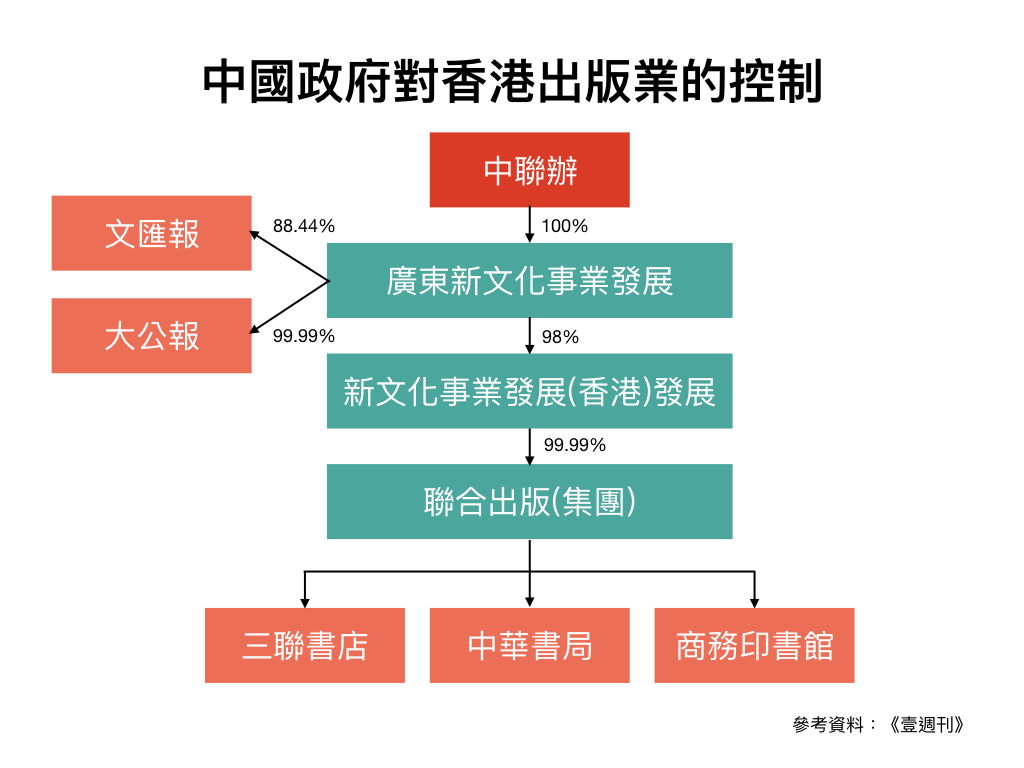
\includegraphics[width=0.7\textwidth]{c28/h-klesson1-045.png}
    \caption{通過中國資本的力量影響輿論} 
\end{figure}

除了業界本身,政府在引導輿論方面同樣有不少改變。各式各樣政治傳訊(甚至有說「政治化妝」)的策略,近年變得越來越普遍。例如因應二十四小時新聞和即時新聞的出現,新聞週期變得越來越短,政府便把一些壞消息留在半夜十二時才以新聞稿的方式發放,使得媒體要立即報道的同時卻無法找到即時回應,到了第二天卻很可能又會有其他新聞覆蓋了這段消息。另一個做法就是一次過把大量有爭議的消息放在同一天內公佈,這樣不單止傳媒機構不會有足夠人手同時深入調查,亦不會有版面作詳細報道,讀者也容易因為信息過於密集而變得麻木。

社會本身的改變,也會使得引導輿論的工作變得容易。社交媒體的興起使得傳播模式由大眾變成分眾,不同興趣立場的人各自去看自己喜歡看的新聞,社會就容易失去共同討論的基礎。而當不同派別的聲音都可以找到討好自己傳媒,無論是建制或非建制陣營的輿論也容易變得極端。社交媒體也會因為收視爭奪戰已變得即時量化,使得煽動情緒的條目就越來越多,慎思明辨和社會責任的考慮就變得次要。

總的來說,CCTVB 所揭示的問題不限於無綫電視這一家企業,而是整個傳媒行業面對的困局。近年漸有新興傳媒出現,意圖以訂閱制或眾籌方式,在中國資本強權下尋找另類的生存空間。然而在資源不足的前提下,要發展出專業的新聞團隊來彌補主流媒體的不足,並不容易。

傳媒行業的困局,本身是整個香港的政治和社會困局的一部分。正如前文所述,當行政權無法代表民意時,公眾便只好向立法權求助;當立法權也無法代表民意時,公眾便再向司法權求助;當司法權也未能滿足民意期望時,公眾便投向大眾傳媒希望他們能為民喉舌。現在連大眾傳媒也失效,是否代表民意的壓力就會隨之而消失?另一個可能,是他們會尋求脫離正規政治的方法發聲,例如走上街頭。



伸延閱讀:

Fung YHA (2007) Political Economy of Hong Kong Media: Producing a Hegemonic Voice, \textit{Asian Journal of Communication 17:2}, p159-171.

Lee FLF (2018) Opinion Media: From Talk Radio to Internet Alternative Websites, \textit{Routledge Handbook of Contemporary Hong Kong}. New York: Routledge.

區家麟,2017,《二十道陰影下的自由:香港新聞審查日常》。香港:中文大學出版社。

梁麗娟(2012):〈大眾傳媒與社會運動的前世今生〉,張少強,梁啟智,陳嘉銘編《香港.論述.傳媒》,香港:牛津大學出版社。